\documentclass{article}
\usepackage{graphicx}
\usepackage{geometry}
\geometry{a4paper, margin=1in}

\title{Heart Disease Data Visualization}
\author{}
\date{}

\begin{document}
	
	\maketitle
	
	\section{Introduction}
	This document presents various visualizations of heart disease data to analyze the relationships between demographics and health metrics, and the distribution of heart disease occurrences.
	
	\section{Gender Distribution of Heart Disease}
	Figure \ref{fig:gender_histogram} shows the histogram of heart disease cases based on gender.
	
	\begin{figure}[h]
		\centering
		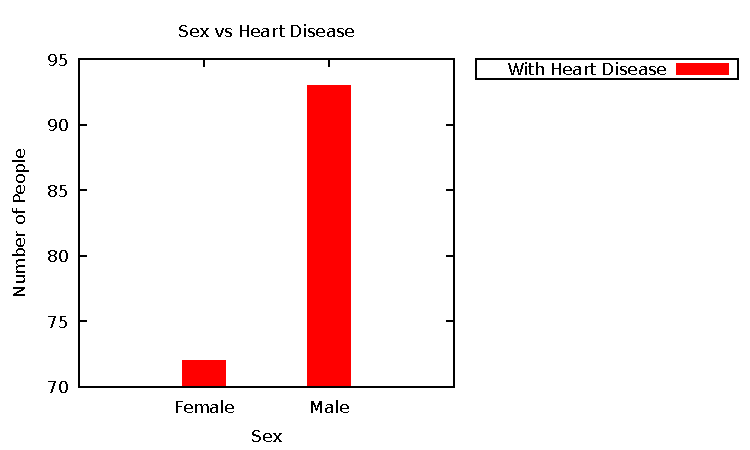
\includegraphics[width=0.8\textwidth]{4a.pdf}
		\caption{Histogram of Gender vs. Number of People with Heart Disease}
		\label{fig:gender_histogram}
	\end{figure}
	
	\section{Correlation Between Age and Health Metrics}
	
	The following figures display correlations between age and specific health metrics, including blood pressure and cholesterol, to help assess risk factors for heart disease.
	
	\subsection{Age vs. Blood Pressure}
	Figure \ref{fig:age_vs_bp} shows a scatter plot of age versus blood pressure, indicating the distribution of blood pressure across different ages.
	
	\begin{figure}[h]
		\centering
		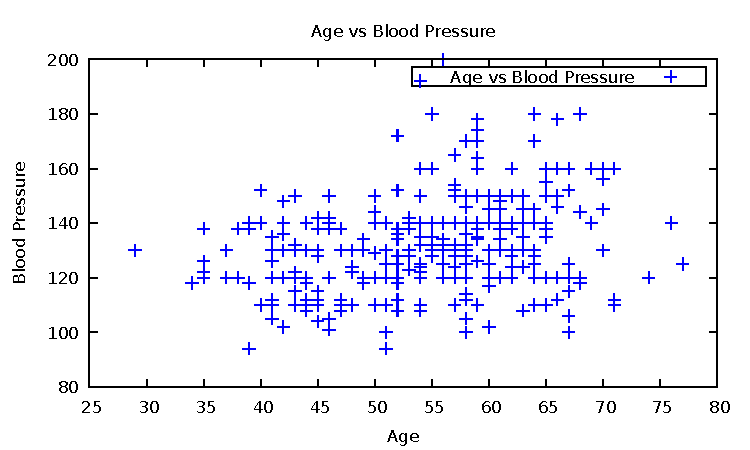
\includegraphics[width=0.8\textwidth]{4b.pdf}
		\caption{Correlation Between Age and Blood Pressure}
		\label{fig:age_vs_bp}
	\end{figure}
	
	\subsection{Age vs. Cholesterol (No Heart Disease)}
	Figure \ref{fig:age_vs_cholesterol} illustrates the correlation between age and cholesterol for those who do not have heart disease, represented by line points.
	
	\begin{figure}[h]
		\centering
		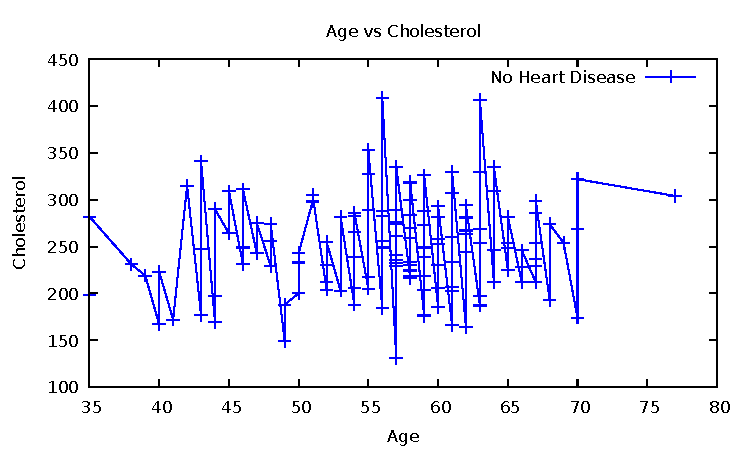
\includegraphics[width=0.8\textwidth]{4c.pdf}
		\caption{Correlation Between Age and Cholesterol (No Heart Disease)}
		\label{fig:age_vs_cholesterol}
	\end{figure}
	
	\section{Age Groups with Heart Disease}
	The pie chart in Figure \ref{fig:age_group_pie} illustrates the percentage of people with heart disease across different age groups. This visualization helps identify the age groups most affected by heart disease.
	
	\begin{figure}[h]
		\centering
		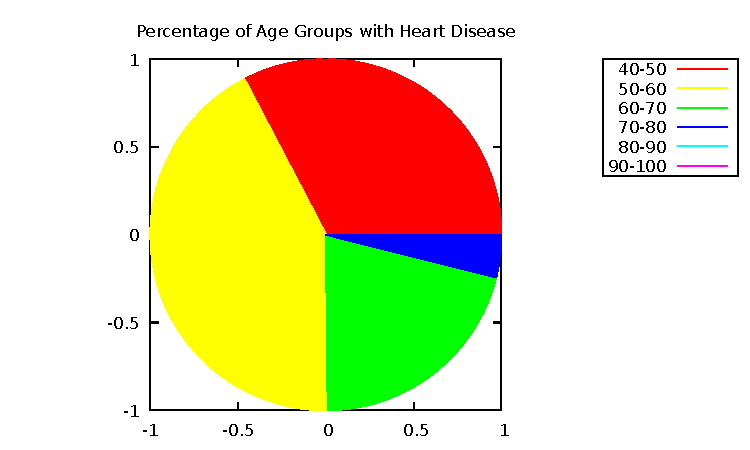
\includegraphics[width=0.8\textwidth]{4d.pdf}
		\caption{Percentage of Age Groups with Heart Disease}
		\label{fig:age_group_pie}
	\end{figure}
	
	\section{Conclusion}
	The visualizations in this document provide insights into the distribution and correlation of heart disease with gender, age, and health metrics like blood pressure and cholesterol. As seen in Figure \ref{fig:gender_histogram}, gender distribution has notable variation, while the correlations shown in Figures \ref{fig:age_vs_bp} and \ref{fig:age_vs_cholesterol} offer insights into health metrics. The pie chart in Figure \ref{fig:age_group_pie} indicates the most affected age groups.
	
\end{document}